\documentclass{article}
\usepackage[margin=25mm]{geometry}
\usepackage{tikz}
\usepackage{hyperref}
\title{Kaggle baselines through canonical HyMeKo IR}
\date{Created: 2026-10-26 03:23 CET}
\begin{document}\maketitle
\paragraph{Scope and acceptance.} Reproduce the official Squares in Squares and Google Quantum AI metrics; construct baseline exports; verify them with unchanged official code; measure one bounded optimization per competition; deliver PDF, CSV/JSON, commands and submission artifacts. Full quantum acceptance requires the official competition data, which currently returns HTTP 401 without local Kaggle credentials. No entry, rule acceptance, submission, publication or Git commit is authorized.
\paragraph{Ownership.} Parser/Core own compilation and canonical IR, reached through the existing local Python facade. Transformation owns the minimal domain projections and experiment composition in tools/kaggle. Official Kaggle code owns validation and scoring. Tensor owns numerical kernels, Graph owns graph searches and spatial hashing, Nagare owns integration/training. The existing P-graph ABB solves a discrete synthesis problem; it is not a continuous packing solver. No second parser, IR builder, general optimizer or ABB engine will be introduced. Source generation is an import/export boundary; search arrays are derived views.
\paragraph{Checkout.} Transformation feat/unversioned at 4f75c1a matches its freshly fetched upstream. Origin/main adds only the merge of this branch. Preserve all existing dirty files. The existing hymeko\_python directory is local-only, with a built native extension and sibling path dependencies: this is local integration evidence, not portable delivery. No new checkout or worktree.
\paragraph{Files and interfaces.} Add this plan, tools/kaggle setup, source pinning, IR projection, packing experiment, quantum preflight/verification adapter, tests, and usage documentation; generated evidence goes under reports/kaggle-20261026. No existing public API or CORE.YAML-protected file changes.
\paragraph{Sequence and budget.} First short correctness tests, then all 1000 packing sizes with resumable per-puzzle checkpoints. Fixed seed 20261026. One CPU worker, 4 GiB sampled RSS limit and 15 minute wall limit per run; no remote computation. Initial estimate: 45--60 minutes for source inspection, implementation, local validation and report; quantum completion depends on data access. Tune only after measuring actual costs.
\paragraph{Verification.} Test exact contact, tiny overlap, rotated geometry, invalid/duplicate IDs, decimal CSV round trip, IR-derived coordinates, source hash enforcement and resume fingerprint. Verify every exported puzzle with the official per-puzzle function and independently re-read the final CSV. Distinguish valid results from the metric's invalid-grid penalty. Compare a fixed-budget grid control with five-square symmetric rotation and shrinking. Keep the best valid incumbent. Report elapsed time and process peak memory separately from objective values.
\paragraph{Quantum gate.} Preserve order, controls, phase and ancilla lifetime through the official kickmix parser before proposing an IR mapping. Do not manufacture circuits, verifier outcomes or baseline costs while the official data is missing. Pin the metric, inventory requirements and make the missing-data condition executable. Full verifier runs retain official sample counts and use explicit local salts, never claiming equivalence to secret leaderboard salts.
\paragraph{Risks and rollback.} All 1000 puzzles contain 500500 squares. Stream per puzzle to bound memory. Exact contacts can make interval validation slow; use a declared tiny grid clearance and test true contacts separately. Reject a failed or unparseable candidate even when its penalty equals the baseline. Detect changed source/configuration on resume. Remove only task-owned new paths to roll back; preserve all previous changes. Consolidate and archive the report at this milestone.
\begin{center}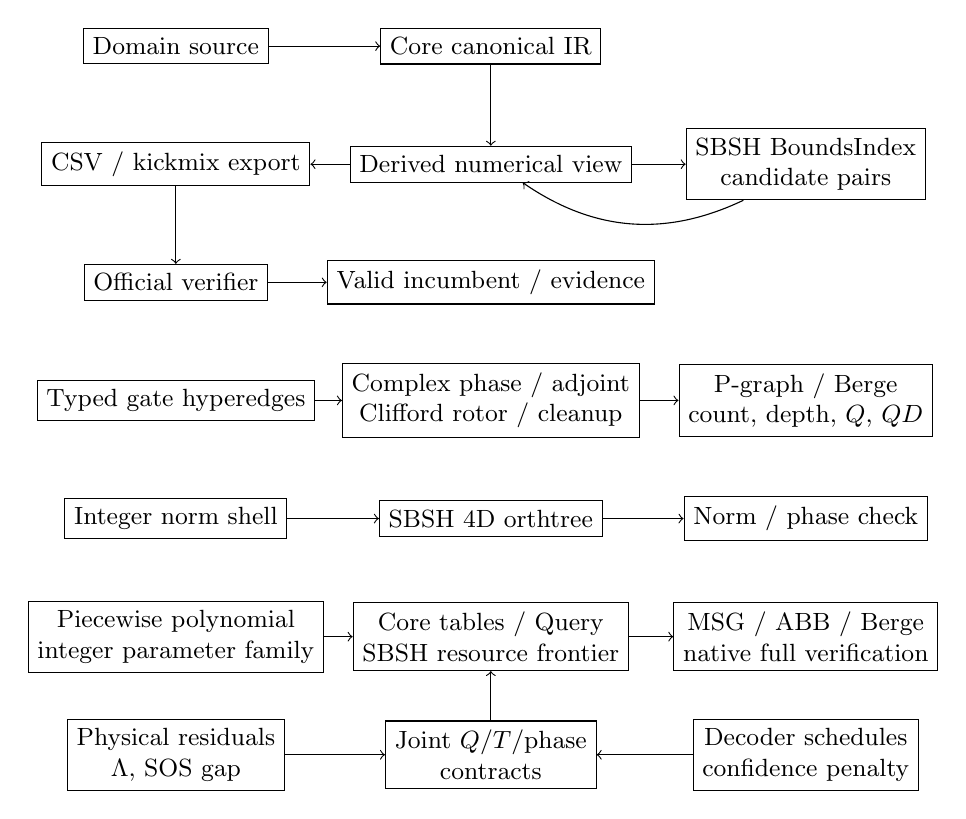
\begin{tikzpicture}[every node/.style={draw,align=center,font=\small}]
\node (src) at (0,0) {Domain source};
\node (ir) at (4,0) {Core canonical IR};
\node (view) at (4,-1.5) {Derived numerical view};
\node (sbsh) at (8,-1.5) {SBSH BoundsIndex\\candidate pairs};
\node (export) at (0,-1.5) {CSV / kickmix export};
\node (verify) at (0,-3) {Official verifier};
\node (record) at (4,-3) {Valid incumbent / evidence};
\draw[->] (src)--(ir);\draw[->] (ir)--(view);\draw[->] (view)--(export);
\draw[->] (view)--(sbsh);\draw[->] (sbsh) to[bend left] (view);
\draw[->] (export)--(verify);\draw[->] (verify)--(record);
\node (gates) at (0,-4.5) {Typed gate hyperedges};
\node (semantics) at (4,-4.5) {Complex phase / adjoint\\Clifford rotor / cleanup};
\node (synthesis) at (8,-4.5) {P-graph / Berge\\count, depth, $Q$, $QD$};
\draw[->] (gates)--(semantics);\draw[->] (semantics)--(synthesis);
\node (lattice) at (0,-6) {Integer norm shell};
\node (ortho) at (4,-6) {SBSH 4D orthtree};
\node (accepted) at (8,-6) {Norm / phase check};
\draw[->] (lattice)--(ortho);\draw[->] (ortho)--(accepted);
\node (nativefamily) at (0,-7.5) {Piecewise polynomial\\integer parameter family};
\node (nativecore) at (4,-7.5) {Core tables / Query\\SBSH resource frontier};
\node (nativeverify) at (8,-7.5) {MSG / ABB / Berge\\native full verification};
\draw[->] (nativefamily)--(nativecore);\draw[->] (nativecore)--(nativeverify);
\node (physical) at (0,-9) {Physical residuals\\$\Lambda$, SOS gap};
\node (jointcost) at (4,-9) {Joint $Q/T$/phase\\contracts};
\node (decoder) at (8,-9) {Decoder schedules\\confidence penalty};
\draw[->] (physical)--(jointcost);\draw[->] (decoder)--(jointcost);
\draw[->] (jointcost)--(nativecore);
\end{tikzpicture}
\end{center}
\section*{SBSH continuation: 26 October 2026, 11:34 CET}
The user explicitly requested continuing the square task with SBSH while away.
Graph's existing \texttt{BoundsIndex} remains the only spatial-index implementation.
Add a thin, bounded binary-stdio example in Graph (no new dependency or algorithm),
and a Python client in the existing Transformation experiment. The client sends
derived AABBs from current square coordinates; Core retains domain identity.
The official SAT supplies the narrow phase and the unchanged official metric
certifies every incumbent/export. Conservative broad-phase candidates are checked
against an independent pairwise AABB oracle, including plane-spanning boxes,
degenerate 2D bounds, exact contact, rotated boxes and rebuilt moving configurations.

Extend the existing five-square family to four $k$-by-$k$ corner blocks and one
central rotated square: $N=4k^2+1$, $k=1,\ldots,15$. Preserve the previous complete
submission as the incumbent and save only the changed models plus a new complete
CSV. Each grid/rotated family uses the same 24-step shrink budget. Run both SBSH
and the official sweep on identical candidates; require identical valid winners.
Measure the two broad phases after warmup over at least five repetitions, including
IPC and rebuild costs; do not attribute geometric gains to the index.

Graph checkout: \texttt{feat/newest-core}, revision \texttt{5693543}, matches its
freshly fetched upstream. Transformation still matches its fetched task branch.
Both dependency audits show a single pinned Core/Parser identity for SBSH.
The old Python binding remains an existing local binary; no unrelated dependency
repair is required across the scalar-buffer process boundary.
Builds reuse the configured machine-wide Cargo intermediate cache.

ETA: about 45 minutes for bridge, tests, bounded comparisons and evidence, with
archival afterward. Each experiment: one logical CPU, 4 GiB sampled process-tree
RSS, 900 seconds maximum. No remote execution, publication or rule acceptance.
Affected paths: Graph's new \texttt{hymeko\_sbsh/examples/bounds\_stdio.rs};
Transformation's existing \texttt{tools/kaggle} experiment and tests, this plan,
and generated \texttt{reports/kaggle-sbsh-20261026}. Preserve the earlier report
and source checksums. Archive one consolidated report after the continuation.
\section*{Quantum continuation: 26 October 2026, 18:29 CET}
The user supplied the official package under
\texttt{01\_analysis/kaggle/google-verifiable-quantum-circuit-compilation}.
It contains all sample circuits and verifiers, the FeMoCo reference integrals,
and a Linux \texttt{kickmix.so}. The loader identifies Python 3.13 as its ABI;
the existing local WSL Ubuntu has Python 3.14. Use an isolated Python 3.13
environment in the WSL user cache, and the unmodified supplied simulator.
No competition data is copied to a public service or modified in place.

Transformation owns the experiment adapter; the supplied generators and verifiers
retain circuit construction and verification semantics. Core retains the domain
model for any selected parameterized optimization; cross-platform execution uses
a derived, hashed configuration, with explicit register, phase and cleanup
contracts. No handwritten kickmix parser or alternate verifier.

First inventory and hash the inputs. Run reduced smoke checks explicitly labeled
as non-scoring, then full official baseline checks for all three tasks. Select one
optimization only after inspecting measured cost breakdowns. Preserve baseline
files and validate the final serialized candidate. Export scores, resource logs,
source provenance and a concise PDF; never infer a private-leaderboard score from
local salts. Technical dependencies and sample counts stay pinned.

Resource budget: one CPU and one verifier worker, up to 8 GiB process-tree memory,
initially 900 seconds per full verification. The DQI documentation estimates about
6 GiB per worker, so the earlier 4 GiB square budget is insufficient here.
Short smoke checks precede expensive runs; adjust a necessary full-run budget only
from measured evidence and record it before execution. No remote computation.
ETA: approximately 60--90 minutes for environment, baseline checks, one bounded
optimization experiment and report, subject to observed full-verifier cost.
The fetched Transformation task branch is current; preserve all unrelated edits.
At 18:45 CET the DQI smoke exceeded 8 GiB (sampled peak 8,595,623,936 bytes)
and the supervisor stopped only its child. Repeat that short smoke at 12 GiB,
one worker, before the full DQI run; about 30 GiB is available in the local WSL VM.
\section*{Typed quantum prototype: 26 October 2026, 21:04 CET}
Implement a bounded, executable prototype in a new domain-owned
\texttt{hymeko\_quantum} crate in Transformation. Parser/Core retain compilation,
IR and identities; Query supplies inherited fields and isa; the existing pinned
Graph and P-graph libraries supply Berge search and ABB. No Graph checkout edits,
second parser, canonical IR builder, or copied search algorithm. The existing
Graph checkout is behind its fetched upstream and has untracked work: consume
the already-published Graph revision pinned by Transformation instead.

Gate instances are typed hyperedges over shared qubit nodes, with explicit
control/target incidence roles and a checked total order. Supported first slice:
X, H, Z, CNOT, CZ and Toffoli, with real amplitudes and phases 0 or pi, at most
8 qubits and 64 gates per circuit. Reject unsupported measurements and arbitrary
rotations. Reverse execution uses inverse gates in reverse order. A declared
clean-ancilla contract is checked on every basis vector of the valid input
subspace, preserving amplitudes and phase, against an independent CZ target.
Track computational-basis Shannon entropy and one-qubit reduced von Neumann
entropies on a declared coherent probe; global pure-state entropy is invariant.

Canonical source also contains a bounded portfolio of implementation edges
between contract boundaries. Verify implementations before admitting them to
P-graph ABB and directed Berge search, including reverse search and entropy
tie-breaking. Gate count is the explicit prototype objective; this is not a
Kaggle score or unrestricted rewrite synthesis. Compare the three-gate
Toffoli--Z--Toffoli implementation with direct CZ and H--CNOT--H; an invalid
identity proposal must be rejected despite its lower cost.

Affected files: workspace Cargo manifest/lock, the new crate's manifest,
library, thin CLI, metamodel, demonstration and integration tests; this existing
plan; one generated prototype report. CORE.YAML changes: none. Preserve all
unrelated dirty files. New dependencies reuse existing pinned Core/Graph/Query
and serde; P-graph is added at the same Graph revision. Audit the selected
dependency closure for duplicate framework identities.

Acceptance: Core CLI compiles every authored model; domain validator rejects
bad roles, aliases, arity, ordering and unsupported gates; exhaustive subspace
equivalence and inverse checks pass; ABB and forward/reverse Berge select the
same valid minimum; entropy trace exposes cleanup; CLI emits replayable JSON.
Focused correctness tests only, no performance campaign. ETA approximately
45--60 minutes including compilation, integration and consolidated evidence.
Runtime bounds: 256 amplitudes, 64 gates/circuit, at most 12 alternatives; no
large competition run. Rollback consists of removing only this new crate and
its named manifest entries, preserving previous experiments and user changes.
\section*{Resource objectives: 27 October 2026, 00:40 CET}
Extend the same bounded quantum owner with a resource projection and four
explicit objectives: gate count, depth, active qubits and logical space--time
volume $Q D$. Unit-duration primitive gates use exclusive qubit access;
disjoint gates may run in parallel while each wire retains authored order.
Depth is the critical path of that fixed dependency graph, not a globally
minimal schedule after commutation rewrites. The static reservation model keeps
all data qubits and every used workspace qubit for the whole circuit. No physical
gate times, hardware connectivity, T decomposition, noise or magic-state factory
model is asserted.

All metrics are computed on the complete verified candidate before passing its
scalar objective to the existing ABB and Berge engines. This is exact for the
current single-stage portfolio; $Q D$ and maxima must not be added over arbitrary
multi-stage compositions. Add a CNOT fanout example on eight arbitrary data
qubits (short star versus conjugated tree), plus a two-phase example comparing
one reused workspace with two concurrent workspaces. The second portfolio is
explicitly restricted to the supplied compute/uncompute implementations; direct
CZ is an independent target, not a claimed global lower bound.

Check complete input-subspace equivalence, inverse, valid layer assignments,
expected independent resource counts and objective-dependent selections. Add
mutations with missing tree preconditioning and shared control/target conflicts.
Reuse the existing 12 correctness tests. Model caps remain unchanged. No runtime
benchmark or remote execution. ETA: about 30 minutes for the focused extension,
small examples, JSON/CSV/plot evidence and archival. Affected files: the quantum
library, models, tests, README; existing report renderer and this plan. No new
dependencies or protected Core edits. Freshly fetched Transformation remains
at 44b1f1f8 on its current task branch; preserve unrelated dirty files.
\section*{Complex operators and phase-preserving rotors: 27 October 2026, 01:24 CET}
Replace the quantum interpreter's real state vectors with one Complex64 execution
path. Real inputs remain convertible at the public boundary. Add S, S-dagger, T,
T-dagger and parameterized U(2)/controlled-U(2) hyperedges. Represent each local
operator as an explicit phase and a unit rotor in the existing published
Clifford algebra. Reuse f64 Multivector geometric multiplication and reversion;
do not copy quaternion multiplication or change Tensor's f32 SO(3) helpers.
Quantum owns the SU(2) embedding and phase contract, Core/Query remain authoritative
for models, and Graph/P-graph remain the search owners.

Add num-complex 0.4.6 as the general complex arithmetic provider and consume the
already pinned hymeko-clifford revision. Discovery found a minimal modal-analysis
Complex in Dynamics, but no general complex scalar facade in Tensor/Core;
depending on Dynamics would also pull the unrelated geometry/physics graph.
No complex arithmetic implementation is copied or introduced in Quantum.
No Tensor or protected Core edits. Audit the selected dependency closure. Preserve
all pre-existing dirty work and prior report snapshots.

Acceptance: all prior 20 tests still pass; independent complex matrix checks
cover T/S adjoints, imaginary input amplitudes and density coherences; Clifford
rotor composition agrees with complex 2x2 multiplication. Preserve q versus -q
unless compensated by the explicit phase. Controlled -I must differ from I.
Compare parameterized targets with elementary gate decompositions through the
same complete-candidate P-graph and Berge paths. Bounds remain 8 qubits, 64 gates,
12 alternatives. No full competition run or performance benchmark.

Kliuchnikov et al. (arXiv:2203.10064v2, Section 4.5) use a Gaussian lattice-volume
heuristic and gate-set-specific arithmetic synthesis. Their approximation-cost
scaling is not an admissible A* remaining-cost bound. This phase establishes the
complex/quaternion semantic boundary required for that synthesis; it does not
claim to implement the paper's integer-lattice enumeration, norm-equation solver
or probabilistic fallback channels. Floating-point rotors do not replace exact
arithmetic over the Clifford+T coefficient ring.

Affected paths: quantum Cargo manifest and workspace lock, local operator module,
existing model/simulator/search/resource modules, metamodel, complex fixtures and
tests, README, the existing report renderer and this plan. Public execute accepts
real or Complex64 input and returns Complex64 output; callers are updated. Record
the inspected literature and the missing synthesis components in the report.
ETA roughly 40 minutes including integration and archival. Rollback removes the
named additions and restores only this phase's edits, preserving all other work.
\section*{SBSH lattice search and official evaluation: 27 October 2026, 01:56 CET}
Use Graph's published N-dimensional integer orthtree for bounded quaternion
norm-shell range queries. Quantum owns exact small-integer shell enumeration,
operator interpretation and the final phase-sensitive acceptance predicate;
SBSH owns partitioning and traversal. Start with the V-basis norm shells
$a^2+b^2+c^2+d^2=5^k$, $0\leq k\leq4$, at most 6248 points. This establishes a
complete bounded search, not a general Clifford+T arithmetic synthesizer.
Unsigned coordinates are a reversible integer shift of the signed coefficients;
half-open query bounds are widened before the exact candidate checks. Compare
the indexed result with full enumeration, including boundaries and phase/sign.
No copied orthtree or consumer-side graph traversal.

Separately produce a real competition candidate if correctness screening admits
one. Inspect FeMoCo angle-word precision and batching using the supplied unchanged
numerical checks and circuit generator. Preserve the factorization weights and
fixed shifts. Never count a numerical screen as quantum verification, never
attribute an unrelated score change to SBSH lattice search, and never overwrite
the existing accepted submission. If a candidate passes, run the official full
task verifier and, for a new selected bundle, the full aggregate metric.

Budgets: small lattice tests bounded by the shell/candidate caps; numerical
screen at most six precisions, one CPU, 4 GiB and 300 seconds; each FeMoCo circuit
check one CPU, 4 GiB and 300 seconds. A full three-task bundle uses the previously
validated one-CPU, 12 GiB, 900-second limit. Keep full shot counts and local salt,
and explicitly distinguish local official-metric values from leaderboard scores.
The user's evening target is a deadline; no delayed or unattended job is assumed.
ETA about 60--90 minutes including implementation, conditional full runs and
archival. No Kaggle submission, publication or remote computation.

Affected files: quantum lattice module, thin CLI, fixtures/tests and manifest;
the existing Kaggle adapter/model/report code, this plan, new artifact/evidence
directories. Reuse current checkouts and pinned dependencies; Graph was fetched
and is read-only. Core/Parser/Query ownership stays unchanged. No CORE.YAML edits.
Required evidence: lossless integer range queries, exact norm certificates,
phase-sensitive acceptance, official candidate verification receipts and hashes.
If no candidate improves, retain and report the incumbent without fabricating a
gain. Norm-shell enumeration does not establish the paper's asymptotic claims.
The first FeMoCo screen rejected brot 11, 10 and 9 (two-body residuals
0.02972, 0.04382 and 0.07871 against the 0.020 threshold); no failed word
proposal is eligible for circuit promotion. Continue the existing inverse-square
root local precision search to its already supported four-round bound, reusing
the official fixed-point model. This is a separate numerical refinement, not an
SBSH-derived score gain. Budget 300 seconds/4 GiB for screening and 900 seconds/
4 GiB for full inverse-square-root verification. Preserve all earlier receipts.
\section*{Native arithmetic synthesis continuation: 27 October 2026}
Created at 03:03 CET. Scope and ownership are recorded in \texttt{synthesis.md}.
Generate direct piecewise polynomial inverse-square-root macros, varying dyadic
segment bits 3--7, degree 2--4 and fractional precision 28--32 (75 candidates).
The new algorithm can replace the Newton square and two multiplications with
lookup and a direct Horner chain. Exact emitted integer arithmetic must pass
every official input before native selection. Core owns each generated table;
Query reads it, SBSH filters resource dominance, and existing MSG/ABB and Berge
select complete contracts. Rebuild the selected native circuit from Core and
require identical bytes before unchanged full official verification.

ETA: approximately 30--45 minutes for integration, focused tests and full native
verification, with a 600-second/4-GiB screening cap and a 900-second/12-GiB
aggregate verification cap, one CPU. A local score is never a leaderboard score.
Preserve prior accepted artifacts; package only after full verification and a
cost improvement. Report and archive the consolidated phase once after writers
finish. No commit, upload or provider-repository mutation is included.
\section*{Three-task physical/resource continuation: 27 October 2026}
Created at 03:45 CET; ETA 45--75 minutes. The bounded plan is recorded in
\texttt{multitask.md}. Refine inverse-square-root coefficients against emitted
integer arithmetic, test shorter coherent DQI schedules against the actual
confidence penalty, and optimize FeMoCo physical factors jointly with QROM
resources. The FeMoCo objective is
$\lambda_{\mathrm{eff}} Q T$, with
$\lambda_{\mathrm{eff}}=\sqrt{E_{\mathrm{gap}}(2\Lambda-E_{\mathrm{gap}})}$.
Keep fixed shifts, energy/norm floors and the 20 mHa error limits unchanged.

Full factor-space rotations preserve the Gram matrix; truncated SVD must pass
physical accuracy again. Quantize the two-body vectors before deriving the
one-body eigensystem. A chunked native unary QROM trades operations for workspace
and must preserve arbitrary XOR targets. Core owns source-bound recipes; Query,
SBSH, MSG/ABB and Berge retain their existing roles. Require identical rebuilt
bytes and full unchanged official verification before promotion. Use up to
600 seconds/4 GiB for numerical screens and 900 seconds/12 GiB for DQI and the
final aggregate, one CPU; avoid concurrent heavy runs. No neural-search,
global-optimality, device-noise or leaderboard claims follow from these tests.
\end{document}
